\chapter{Fase di ricerca}

Parte della ricerca si è basata sullo studio degli algoritmi utilizzati, e precisamente:
\begin{itemize}
    \item perché e quando sono stati creati,
    \item da chi sono stati prodotti,
    \item a quali bisogni rispondono,
    \item da chi sono stati utilizzati nel tempo.
\end{itemize}
Inoltre, è stato condotto un esperimento per determinare se vi fosse una dipendenza effettiva tra i vari frame dei light field e se tale dipendenza potesse influenzare la qualità complessiva della compressione/decompressione.
\\
Infine, è stata preparata una tabella riassuntiva per evidenziare le peculiarità fondamentali per la comprensione dei risultati del progetto. Ulteriormente, sono stati esaminati il Structural Similarity Index (SSIM) e il Peak Signal-to-Noise Ratio (PSNR), due metodi utilizzati per valutare la qualità percepita delle immagini in scenari di compressione lossy.

\clearpage
\section{Tabella riassuntiva}
\begin{table}[ht]
    \centering
     \begin{tabular}{|c|c|c|}
        \hline
        Codec & Licenza & Perdita \\
        \hline
        Cirrus Logic & Commerciale & Lossy \\
        FLV & GNU & Lossy \\
        MJPEG & GNU & Lossy \\
        MPEG4 & GNU & Lossy \\
        ProRes & Commerciale & Lossy \\
        \hline
        FFVHUFF & GNU & Lossless \\
        LCL-ZLIB & GNU & Lossless \\
        MAGICYUV & Commerciale & Lossless \\
        \hline
    \end{tabular}
    \label{tab:RecapTable}
\end{table}

\subsection{Cirrus Logic AccuPak}
Cirrus Logic AccuPak è un codec YUV a precisione ridotta.
\\
\\
Il codec AccuPak racchiude 4 campioni Y e 2 campioni C in 32 bit rappresentando ogni campione Y con 5 bit e ogni campione C con 6 bit. È essenzialmente un metodo ridimensionato di codifica YUV 4:1:1, in cui ogni gruppo di 4 pixel su una linea è rappresentato da un campione di luminanza ciascuno ma condivide campioni C\cite{CirrusLogicAccuPak}.

\subsection{FLV}
Flash Video è un formato di file utilizzato per fornire contenuti video digitali (ad esempio, programmi TV, film, ecc.) su Internet utilizzando Adobe Flash Player versione 6 e versioni più recenti. Il contenuto Flash Video può anche essere incorporato nei file SWF. Ci sono due diversi formati di file Flash Video: FLV e F4V. I dati audio e video all'interno dei file FLV sono codificati allo stesso modo dei file SWF. FLV è stato originariamente sviluppato da Macromedia. Nei primi anni 2000, Flash Video era lo standard de facto per lo streaming video basato sul web (su RTMP).
\\
\\
I file Flash Video FLV di solito contengono materiale codificato con codec che seguono i formati di compressione video Sorenson Spark o VP6. A partire dal 2010 le versioni pubbliche di Flash Player (collaborazione tra Adobe Systems e MainConcept) supportano anche il video H.264 e l'audio HE-AAC. Tutti questi formati di compressione sono limitati dai brevetti. Flash Video è visualizzabile sulla maggior parte dei sistemi operativi tramite Adobe Flash Player e il plugin del browser web o uno dei numerosi programmi di terze parti. I dispositivi iOS di Apple, insieme a quasi tutti gli altri dispositivi mobili, non supportano il plugin Flash Player e quindi richiedono altri metodi di consegna come quelli forniti da Adobe Flash Media Server\cite{FLV}.

\subsection{Motion JPEG}
Motion JPEG (M-JPEG) è un codec video nel quale ogni singolo frame del video viene compresso in un'immagine JPEG.
\\
Non offre nessuna compressione interframe, questo fa sì che la qualità della compressione sia indipendente dal movimento presente nell'immagine, a differenza della compressione MPEG dove ci possono essere problemi di qualità quando il video contiene movimenti veloci o cambi scena. Questo codec facilita il montaggio video, in quanto permette tagli su ogni singolo frame, e non solo all'inizio di un gruppo di frame.
\\
Si tratta di un formato che ha avuto una certa diffusione su fotocamere digitali e camere IP in quanto permetteva di usare la tecnologia della compressione JPEG anche per i filmati. Pur richiedendo un bitrate superiore al formato MPEG-1 permette risoluzioni superiori. È stato gradualmente soppiantato dai formati MOV(Apple), MPEG-2 e MPEG-4\cite{M-JPEG}.

\subsection{MPEG4}
In elettronica e telecomunicazioni MPEG-4, nato nel 1996 e finalizzato nel 1998 (fu presentato pubblicamente a settembre di quell'anno), è il nome dato a un insieme di standard per la codifica dell'audio e del video digitale sviluppati dall'ISO/IEC Moving Picture Experts Group (MPEG). L'MPEG-4 è uno standard utilizzato principalmente per applicazioni come la videotelefonia e la televisione digitale, per la trasmissione di filmati via Web, e per la memorizzazione su supporti CD-ROM.
\\
MPEG-4 è suddiviso in vari sotto standard chiamati part (termine inglese che in italiano significa "parte") e noi abbiamo usato la parte 2: un codec di compressione per i dati visivi (video, still textures...). Uno dei tanti "profili" della parte 2 è il Advanced Simple Profile (ASP).
\\
\\
Il concetto alla base del codec (COdificatore-DECodificatore) MPEG-4 è la quantizzazione. Senza scendere nello specifico, si può riassumere come quel processo che permette di trasmettere solamente la variazione dell'immagine mediante un apposito algoritmo di compressione\cite{MPEG-4}.

\subsection{ProRes}
Apple ProRes è un formato di compressione video lossy di alta qualità, "visually lossless" sviluppato da Apple Inc. per l'uso in post-produzione che supporta una risoluzione video fino a 8K. È il successore dell'Apple Intermediate Codec ed è stato introdotto nel 2007 con Final Cut Studio 2. Proprio come gli standard H.26x e MPEG, la famiglia di codec ProRes utilizza algoritmi di compressione basati sulla trasformata del coseno discreto (DCT). ProRes è ampiamente utilizzato come metodo di consegna del formato finale per i file di trasmissione HD in pubblicità, funzionalità, Blu-ray e streaming.
\\
\\
ProRes è una linea di codec intermedi, il che significa che sono destinati all'uso durante l'editing video e non alla visualizzazione pratica da parte dell'utente finale. Ciò si ottiene utilizzando solo la compressione intra-frame, dove ogni fotogramma viene memorizzato in modo indipendente e può essere decodificato senza dipendenze da altri fotogrammi. Il vantaggio di un codec intermedio è che offre eccellenti prestazioni di accesso casuale nelle applicazioni di post-produzione e mantiene una qualità superiore rispetto ai codec dell'utente finale, pur richiedendo sistemi disco molto meno costosi rispetto ai video non compressi. È paragonabile al codec DNxHD o CineForm di Avid che offrono bitrate simili e sono anche destinati ad essere utilizzati come codec intermedi. ProRes è un codec solo intra-frame basato su scalare DCT ed è quindi più semplice da decodificare rispetto ai formati orientati alla distribuzione come H.264. Nel 2018 Apple ha aggiunto un nuovo "ProRes RAW" (filtro Bayer compresso) a Final Cut Pro X, dopo che Blackmagic Design ha implementato Bayer compresso come "CinemaDNG 3:1" e "CinemaDNG 4:1" nelle loro fotocamere e DaVinci Resolve\cite{ProRes}.


\subsection{FFVHUFF}
FFVHUFF è un codec video senza perdita di dati ed è una versione migliorata, e più veloce, del codec huffyuv. Può gestire più formati pixel\cite{ffvhuff}.

\subsection{LCL-ZLIB}
Il codec converte i dati dell'immagine RGB24 originali in uno spazio colore di destinazione e lo comprime con un algoritmo selezionato. Il codec può anche rimuovere i fotogrammi invariati e sostituirli con fotogrammi nulli e può filtrare i dati dell'immagine prima della compressione. L'unica differenza tra avimszh e avizlib è nel compressore di flusso. Il filtraggio PNG è disponibile solo in avizlib. Fatta eccezione per i frame nulli, non c'è compressione temporale, e tutti i frame possono essere decodificati indipendentemente dagli altri. Ogni blocco AVI contiene un fotogramma. In caso di modalità multithread, le due sezioni sono memorizzate nello stesso blocco.
\\
Come suggerisce il nome del codec, tutti i compressori sono lossless.
\\
Questa modalità utilizza il metodo standard di sgonfiamento zlib. Per la descrizione dell'algoritmo fare riferimento ai documenti zlib. Lo stato del compressore viene reimpostato ogni fotogramma (decodifica ogni fotogramma in modo indipendente). I codici di compressione (1, 9, -1) hanno lo stesso significato dei flag di compressione zlib. Zlib non richiede un livello di compressione al decompressore, quindi il valore è lì solo a scopo informativo\cite{zlib}.

\subsection{MagicYuv}
Un codec video ad alte prestazioni, ultraveloce e matematicamente senza perdite per la registrazione, l'archiviazione, la post-produzione e l'editing ad alte risoluzioni.
\\
MagicYUV è stato progettato per la velocità e per supportare pienamente la codifica e la decodifica multi-thread.
\\
Questo codec è utilizzato per:
\begin{itemize}[noitemsep]
    \item Gaming
    \item Registrazioni e catture
    \item Editing e post-produzione
    \item Ricerca
\end{itemize}
Il Codec MagicYUV consente ai ricercatori di catturare ed elaborare video alle più alte risoluzioni e framerate possibili, in profondità di bit regolari e a colori profondi, mantenendo intatta ogni bit delle informazioni.
\\
Questo rende MagicYUV uno dei codec video lossless più veloci del suo genere\cite{magicyuv}.


\section{Metriche selezionate per il confronto}

\subsection{SSIM}
L'indice SSIM (Structural Similarity Index Measure) è un modello basato sulla percezione che valuta la degradazione dell'immagine considerando i cambiamenti nella percezione delle informazioni strutturali. Questo metodo tiene conto di importanti fenomeni basati sulla percezione, come il mascheramento della luminanza e il mascheramento del contrasto. Il termine "informazioni strutturali" si riferisce ai pixel fortemente interdipendenti o spazialmente vicini, enfatizzando la correlazione tra di essi.
SSIM stima la qualità percepita di immagini e video. Misura la somiglianza tra due immagini: l'originale e la recuperata\cite{sara2019image}.

In particolare, date due immagini o segnali $N$-dimensionali (o porzioni corrispondenti), $x = (x_1, \ldots, x_N)$ e $y = (y_1, \ldots, y_N)$, l'indice SSIM esamina le similarità tra luminanza, contrasto e struttura.

1. Per la luminanza, $l(x, y)$, si utilizzano i valori medi, ad esempio,
\[
\bar{x} = \frac{1}{N} \sum_{i=1}^{N} x_i.
\]

2. Per il contrasto, $c(x, y)$, si utilizzano le varianze, ad esempio,
\[
s_x^2 = \frac{1}{N-1} \sum_{i=1}^{N} (x_i - \bar{x})^2.
\]

3. Per la struttura, $s(x, y)$, si utilizzano segnali normalizzati (deviazione standard unitaria), ad esempio,
\[
x' = \frac{x - \bar{x}}{s_x}.
\]

Successivamente, si combinano questi componenti (in qualche modo!) per ottenere una misura complessiva di similarità, cioè,
\[
S(x, y) = F(l(x, y), c(x, y), s(x, y)).
\]

\subsection{PSNR}
Il PSNR (Peak Signal-to-Noise Ratio) è una metrica utilizzata per calcolare il rapporto tra la potenza massima del segnale possibile e la potenza del rumore di distorsione che influisce sulla qualità della sua rappresentazione. Questo rapporto tra due immagini viene misurato in decibel per tener conto della vasta gamma dinamica dei segnali, che variano dai valori più grandi a quelli più piccoli.
Il PSNR viene comunemente calcolato come il logaritmo in scala decibel, poiché i segnali hanno una gamma dinamica estesa. Questa gamma dinamica riflette la variazione tra i valori più alti e più bassi possibili, che sono critici per valutare la qualità dell'immagine in termini di fedeltà alla sua rappresentazione originale.
Utilizzato ampiamente come tecnica di valutazione della qualità, il PSNR misura la qualità della ricostruzione nei codec di compressione delle immagini lossy. In questo contesto, il segnale rappresenta i dati originali, mentre il rumore è l'errore introdotto dalla compressione o dalla distorsione. 
\\
\\
Nel degrado della qualità della compressione dell'immagine e del video, il valore PSNR varia da 30 a 50 dB per la rappresentazione dei dati a 8 bit e da 60 a 80 dB per i dati a 16 bit.
\\
\\
Il PSNR è espresso come:
\\
\centerline{$PSNR = 10log_{10}(peakval^2) / MSE$}
\\
\\
Qui, peakval (Peak Value) è il massimo nei dati dell'immagine. Se si tratta di un tipo di dati intero senza segno a 8 bit, il peakval è 255. Dall'equazione, possiamo vedere che è una rappresentazione dell'errore assoluto in dB\cite{sara2019image}.

\begin{figure}[!ht]
    \centering
    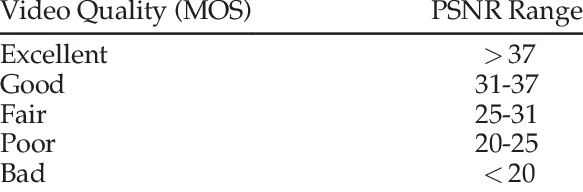
\includegraphics[width=0.40\textwidth]{img/PSNR table.png}
    \caption{Rapporto tra PSNR e qualità del video}
    \label{fig:PSNR-table}
\end{figure}


Nel paper "Social-Aware Video Multicast Based on Device-to-Device Communications" \cite{Social-Aware}, viene condotto uno studio che esamina il rapporto tra la qualità del video e il valore dell'indice PSNR. La Tabella \ref{fig:PSNR-table} fornisce una guida per interpretare i valori di PSNR e associarli a diverse categorie di qualità video. In particolare, si osserva che una qualità del video superiore è indicata da valori di PSNR pari o superiori a 37, mentre una qualità inferiore è associata a valori di PSNR inferiori a 25.
\\
\\
Nella fase di analisi dei risultati, la Tabella \ref{fig:PSNR-table} sarà utilizzata come riferimento per valutare la qualità dei video decompressi. In altre parole, i valori ottenuti durante l'esperimento saranno confrontati con i range indicati nella tabella per determinare se la qualità del video è considerata ottima, buona, accettabile o pessima, in base ai criteri definiti dagli intervalli di PSNR.

\subsection{Test indice SSIM con riferimento}
Per valutare l'accuratezza del calcolo dell'indice di similarità strutturale (SSIM) nel nostro lavoro, è stato condotto un confronto con i valori riportati nel paper di riferimento \textit{"The SSIM Index for Image Quality Assessment"} \cite{TEST_SSIM}. A tale scopo, le stesse immagini utilizzate nel paper di riferimento sono state scaricate e utilizzate per il calcolo dell'indice SSIM mediante uno script personalizzato basato sulla libreria \textit{skimage.metrics}. I valori ottenuti da questo script sono stati quindi confrontati con quelli riportati nel paper di riferimento.
\subsubsection{Risultati}
Il confronto tra i valori SSIM ottenuti dal nostro script e quelli riportati nel paper di riferimento ha mostrato una buona corrispondenza tra i due. Tuttavia, è stato osservato un errore medio relativo, calcolato come la media delle differenze percentuali tra i valori calcolati e quelli di riferimento, pari a \textbf{0.030}.
Questo risultato suggerisce che il nostro script per il calcolo dell'indice SSIM ha una precisione accettabile e può essere considerato affidabile per valutazioni quantitative della qualità delle immagini.

\subsection{Test indice PSNR con riferimento}
Per valutare l'accuratezza del calcolo del PSNR, sono state selezionate due immagini - l'originale e quella con rumore - estratte dalla pagina web specificata \cite{PSNR-HVS}, la quale fa riferimento a due paper accademici. Successivamente, utilizzando le informazioni fornite in questi paper, il PSNR è stato calcolato per le due immagini mediante l'utilizzo di uno script apposito che testa la funzione per il calcolo del PSNR fornita dalla libreria \textit{skimage.metrics} e usata nell'esperimento.

\subsubsection{Risultati}
I valori del PSNR ottenuti sono stati confrontati con quelli riportati sulla pagina web di riferimento, che fornisce i valori di PSNR associati alle immagini specificate. Questo confronto ha permesso di determinare l'errore relativo del PSNR, risultato essere dello 0.026\%. Questo risultato indica che vi è una buona corrispondenza tra i valori calcolati utilizzando la funzione di calcolo del PSNR fornita dalla libreria skimage.metrics e quelli riportati sulla pagina web di riferimento, confermando l'accuratezza del calcolo del PSNR.